\documentclass[captions=tableheading,
  bibliography=totoc,
  titlepage=firstiscover
  ]{scrartcl}
\usepackage{scrhack}

\usepackage[a4paper,top=2.5cm,left=2.5cm,right=2cm,bottom=3cm,bindingoffset=5mm]{geometry}

\usepackage[aux]{rerunfilecheck}

\usepackage{polyglossia}
\setmainlanguage{german}

\usepackage{amsmath}
\usepackage{amssymb}
\usepackage{mathtools}

\usepackage{fontspec}

\usepackage{biblatex}
\addbibresource{lit.bib}  %nach polyglossia

\usepackage[
  math-style=ISO,
  bold-style=ISO,
  sans-style=italic,
  nabla=upright,
  partial=upright,
]{unicode-math}

\usepackage[
  locale=DE,
  separate-uncertainty=true,
  per-mode=symbol-or-fraction,
]{siunitx}

\usepackage[section, below]{placeins}
\usepackage[
  labelfont=bf,        % Tabelle x: Abbildung y: ist jetzt fett
  font=small,          % Schrift etwas kleiner als Dokument
  width=0.9\textwidth, % maximale Breite einer Caption schmaler
  format=plain,
  indention=1em, % Abbildung sticht links etwas hervor
]{caption}
\usepackage{graphicx}
\usepackage{grffile}
\usepackage{subcaption}

\usepackage{booktabs}
\usepackage{float}
\floatplacement{figure}{htbp}
\floatplacement{table}{htbp}


\usepackage[unicode]{hyperref}
\usepackage{bookmark}
\usepackage{microtype}


\title{V203 - Verdampfungswärme und Dampfdruckkurve}
\author{Julian Jung \\ julian.jung@tu-dortmund.de
  \and Pascal Gutjahr \\ pascal.gutjahr@tu-dortmund.de}
  \date{Durchführung: 11.11.2016
  \hspace{3em}
  Abgabe: 18.11.2016}
  \begin{document}
\maketitle
\newpage
\tableofcontents
\newpage
\section{Zielsetzung}
Ziel des Versuchs ist es die Verdampfungswärme L von Wasser zu Untersuchen.
Dafür wird der Druck und die Temperatur untersucht. Im ersten Teil des Versuchs
wird die Verdampfungswärme für niedrigen Druck $(p\le 1$ bar) untersucht. In
diesem Bereich ist L beinahe konstant. In einem zweiten Versuch wird der Zusammenhang
zwischen Druck und Temperatur bei 1 bar < $p$ < 15 bar untersucht.
\section{Theorie}
\section{Aufbau und Durchführung}
\section{Auswertung}
\subsection{p < 1 bar}
Um die Verdampfungswärme L zu berechnen, wird die Formel
\begin{equation*}
  \ln \bigl(\frac{p}{p_0}\bigr)=-\frac{\symup{L}}{\symup{R}} \cdot \frac{1}{\symup{T}}
  %schon verwendet?
\end{equation*}
verwendet. Hierbei ist $p_0$ der Umgebungsdruck und beträgt
\begin{equation*}
  p_0=995\cdot 10^2 \si{\pascal}.
\end{equation*}
Die in Tabelle\ref{tab:data1} gemessenen Werte für den Druck werden logarithmiert und in einem
Diagramm gegen den Kehrwert der absoluten Temperatur aufgetragen.
  \begin{table}
    \centering
    \caption{Messung bis 1 bar}
    \label{tab:data1}
    \begin{tabular}{c c c c}
      \toprule
      T/°C & P/bar & T/°C & P/bar
      \\
      \midrule
      52    &   137  &  76  &  400  \\
      53    &   146  &  77  &  417  \\
      54    &   153  &  78  &  439  \\
      55    &   160  &  79  &  454  \\
      56    &   167  &  80  &  474  \\
      57    &   174  &  81  &  490  \\
      58    &   183  &  82  &  515  \\
      59    &   191  &  83  &  532  \\
      60    &   200  &  84  &  555  \\
      61    &   209  &  85  &  577  \\
      62    &   219  &  86  &  600  \\
      63    &   229  &  87  &  625  \\
      64    &   239  &  88  &  650  \\
      65    &   249  &  89  &  666  \\
      66    &   261  &  90  &  702  \\
      67    &   271  &  91  &  726  \\
      68    &   286  &  92  &  756  \\
      69    &   299  &  93  &  780  \\
      70    &   311  &  94  &  807  \\
      71    &   325  &  95  &  837  \\
      72    &   339  &  96  &  881  \\
      73    &   352  &  97  &  912  \\
      74    &   369  &  98  &  947  \\
      75    &   384  &  99  &  988  \\
      %Wert für 100°C fehlt wegen Formatierung
      \bottomrule
    \end{tabular}
  \end{table}

\begin{figure}[H]
  \centering
  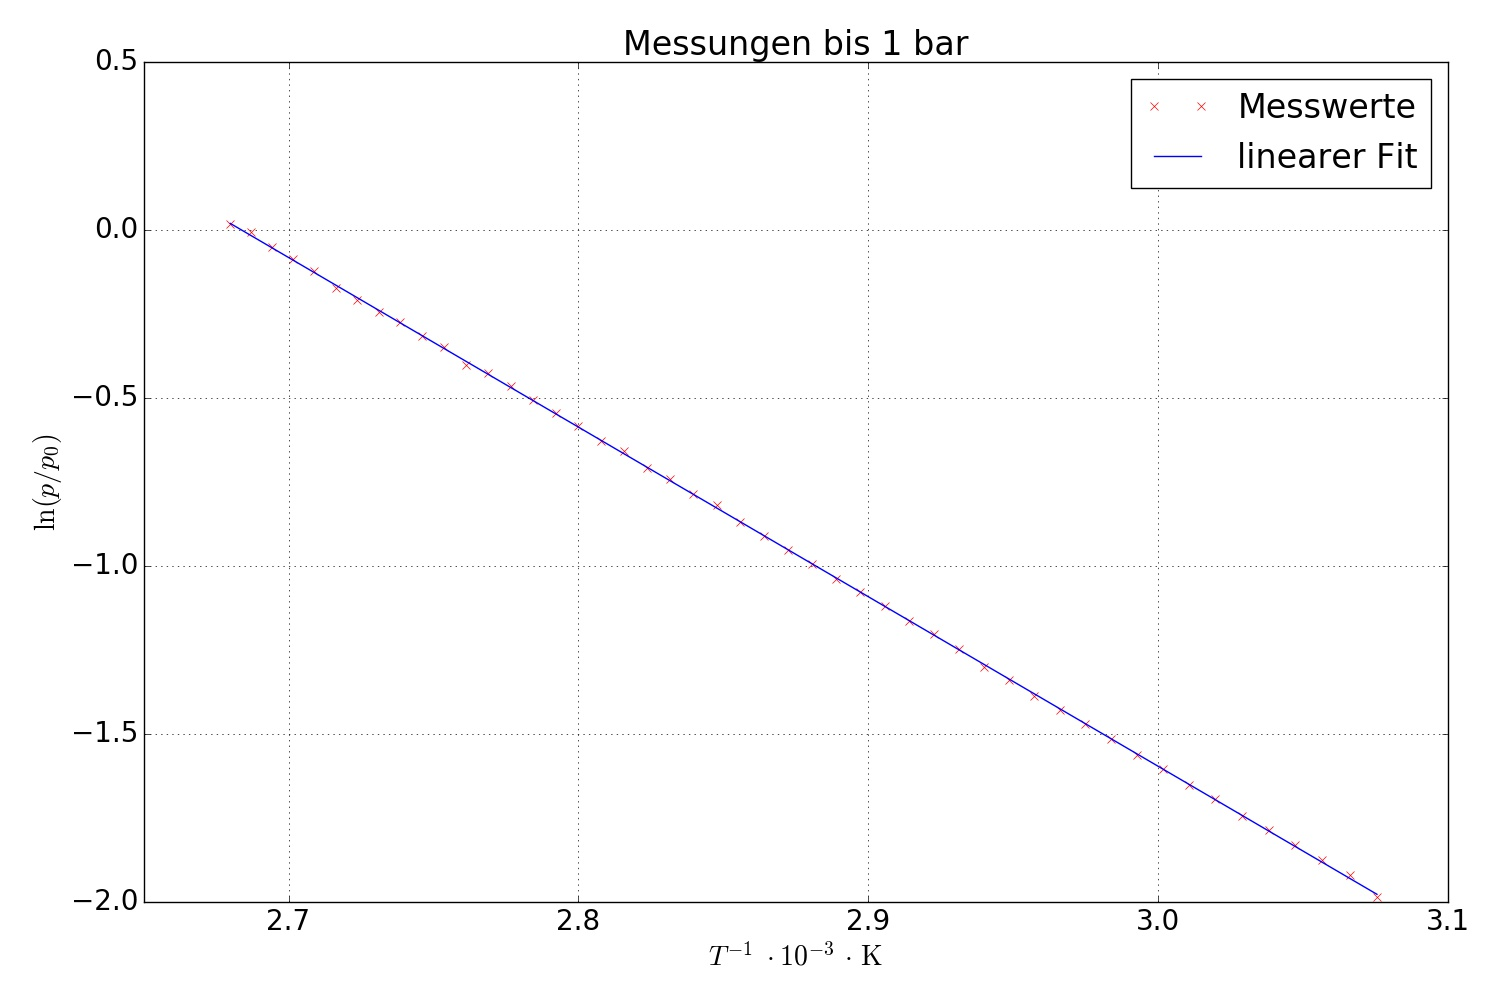
\includegraphics[height=9cm , width=13.5cm]{fit1.jpg}
  \caption{fit1}
  \label{fig:fit1}
  \end{figure}
Die Parameter der linearen Regression werden mit Python 3.5.2 berechnet und
lauten:
\begin{align*}
  a =& (-5,044 \pm 0,006) \cdot 10^3 \si{\kelvin} \\
  b =& (13,54 \pm 0,02)
\end{align*}
Unter Verwendung von Formel \eqref{eq:4} und der allgemeinen Geradengleichung
lässt sich L mit
\begin{equation}
  a=-\frac{L}{\symup{R}} \iff L = -a \cdot \symup{R}
\end{equation}
darstellen. Der dazugehörige Fehler wird über die Gaußsche Fehlerfortpflanzung
berechnet und liefert:
\begin{equation}
  \Delta f = \sqrt{-\symup{R}^2 \cdot \Delta a^2}.
\end{equation}
Wobei R die allgemeine Gaskontante und $\Delta a$ der Fehler von $a$ ist.
Somit ergibt sich:
\begin{equation*}
  L=(41,94 \pm 0,05)\cdot 10^3 \frac{\si{\joule}}{\si{\mol}}.
\end{equation*}
% \newpage
Weiter soll die äußere Verdampfungswärme $L_a$, also die Energie, welche
benötigt wird um das Volumen der Flüssigkeit auf das Volumen des Gases
zu bringen, berechnet werden. Hierbei wird eine Volumenarbeit $W=pV$ geleistet.
Über gleichsetzen der idealen Gasgleichung \eqref{eq:ideal} mit der
Volumenarbeit, lässt sich $L_a$ für eine Temperatur von $T=373 \si{\kelvin}$
berechnen:
\begin{align*}
  L_a =& W =pV=RT \\
      =& 3,10 \cdot 10^3 \si{\joule \per \mol}
\end{align*}
Die innere Energie $L_i$ muss aufgebracht werden, um die molekularen
Anziehungskräfte zu überwinden. Diese ist
\begin{align*}
  L_i=&L-L_a \\
  =& (38,84 \pm 0,05)\cdot 10^3 \si{\joule\per\mol}.
\end{align*}
 Die innere Energie pro Molekül erhält man durch die Division mit der Avogadrokonstanten
 $\symup{N_A}=6,022 \cdot 10^{23} \frac{1}{\si{\mol}}$.
 Dieses Ergebnis wird der Anschaulichkeit halber in Elektronenvolt angegeben
 ($1\si{\electronvolt}=1,602\cdot 10{{-19}}\si{\joule})$.
 Der Fehler wird erneut über die Gaußsche Fehlerfortpflanzung berechnet:
 \begin{equation*}
   \Delta f=\sqrt{\frac{1}{\symup N_A^2}\cdot 0,050^2}.
 \end{equation*}
 Somit:
 \begin{align*}
   L_i =&(4,03\cdot 10^{-4} \pm 1\cdot 10^{-6})\ \si{\electronvolt} \\
   L_i =&(0,403 \pm 0,001) \ \si{\milli\electronvolt}
 \end{align*}
\subsection{p > 1 bar}
Um die Verdampfungswärme, bei höheren Drücken, in Abhängigkeit der Temperatur zu
ermitteln, benötigen wir die Clausis-Clapeyronsche Gleichung (\ref{eq:clausius}).
Diese wird nach der Verdampfungswärme L umgeformt:
\begin{equation}
  L = (V_D - V_F) \;T\; \frac{dp}{dT} \label{eq:8}
\end{equation}
$V_F$ kann hierbei weiterhin vernachlässigt werden, $V_D$ kann nun jedoch nicht mehr
mit der allgemeinen Gaslgeichung (\ref{eq:ideal}) bestimmt werden.
Eine Gute Näherung ist durch die Gleichung
\begin{align}
  \biggr(p + \frac{A}{V^2}\biggl) \; V = RT \qquad mit \qquad A = 0,9 \frac{\si{\joule \meter^3}}
  {\si{\mol^2}}
\end{align}
gegeben.
Diese Gleichung wird dann nach $V_D$ umgeformt:
\begin{equation}
  V_D = \frac{RT}{2p} \pm \sqrt{\biggr(\frac{RT}{2p}\biggl)^2-\frac{A}{p}}
\end{equation}
Anschließend wird dieser Term in (\ref{eq:8}) eingesetzt:
\begin{equation}
  L = \Biggr(\; \frac{RT}{2p} \pm \sqrt{\biggr(\frac{RT}{2p}\biggl)^2-\frac{A}{p}} \; \Biggl)
  \; T \; \frac{dp}{dT}
\end{equation}
Für die Lösung von $\frac{dp}{dT}$ wird ein Ausgleichpolynom 3. Grades verwendet,
\begin{align}
  p(T) &= a \cdot T^3 + b \cdot T^2 + c \cdot T + d  \label{eq:pt}\\
  \frac{dp}{dT} &= 3a \cdot T^2 + 2b \cdot T +    \label{eq:dp}
\end{align}
mit den Parametern:
\begin{align*}
  a &= (0,009 \pm 0,001) \; \si{\frac{\pascal}{\kelvin^3}} \\
  b &= (-11 \pm 1) \; \si{\frac{\pascal}{\kelvin^2}} \\
  c &= (4,3 \pm 0,6) \; \cdot 10^3 \; \si{\frac{\pascal}{\kelvin}} \\
  d &= (-5,6 \pm 0,8)\; \cdot 10^5 \; \si{\pascal}
\end{align*}

\begin{table}
  \centering
  \caption{Messung bis 15 bar}
  \label{tab:data2}
\begin{tabular}{c c c c}
  \toprule
  T/\si{\celsius} &   P/\si{\bar}  &   T/\si{\celsius} &   P/\si{\bar} \\
  \midrule
  100  &   2.24   &   132  &   4.69  \\
  102  &   2.33   &   134  &   4.94  \\
  104  &   2.43   &   136  &   5.20  \\
  106  &   2.54   &   138  &   5.48  \\
  108  &   2.66   &   140  &   5.78  \\
  110  &   2.78   &   142  &   6.11  \\
  112  &   2.90   &   144  &   6.48  \\
  114  &   3.04   &   146  &   6.87  \\
  116  &   3.18   &   148  &   7.31  \\
  118  &   3.34   &   150  &   7.79  \\
  120  &   3.50   &   152  &   8.36  \\
  122  &   3.67   &   154  &   9.03  \\
  124  &   3.85   &   156  &   9.81  \\
  126  &   4.04   &   158  &  10.86  \\
  128  &   4.25   &   160  &  12.26  \\
  130  &   4.47   &   162  &  14.46  \\
  \bottomrule
  \end{tabular}
\end{table}

\begin{figure}[H] % ein großes H steht dafür, dass das Objekt auf jeden Fall den Platz hält
  \centering
  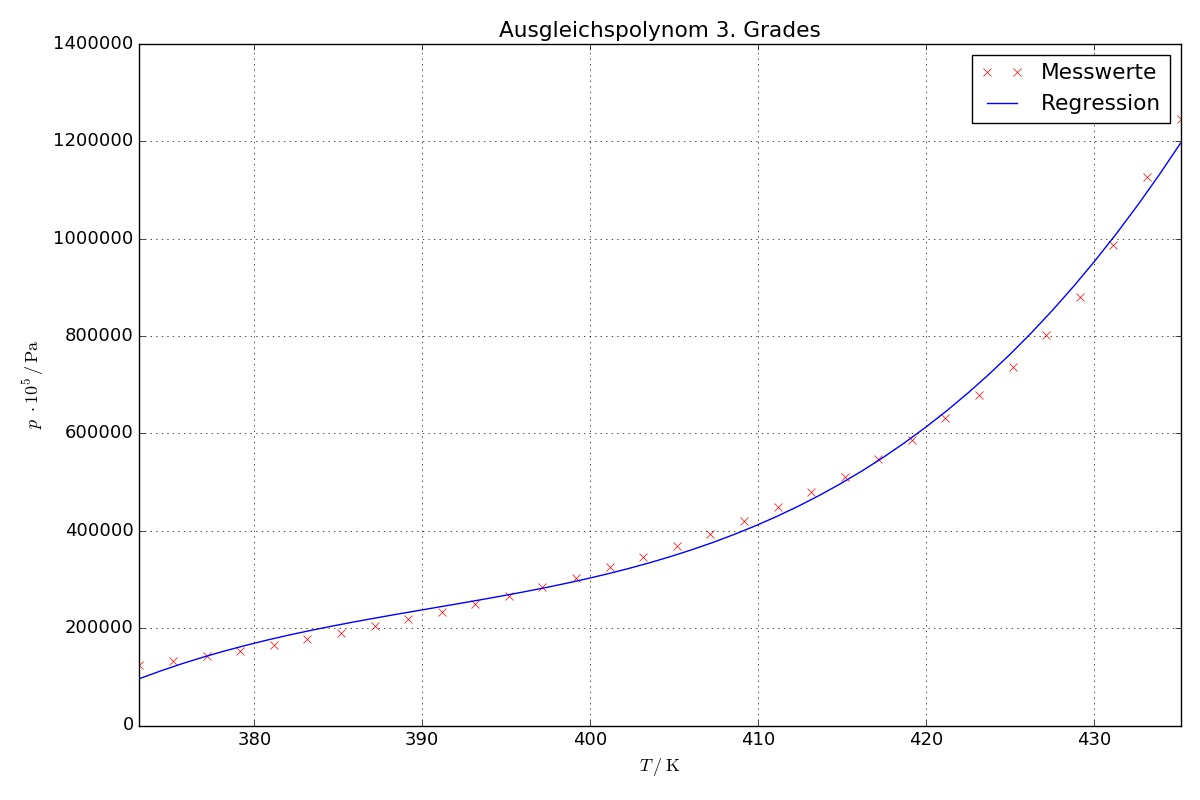
\includegraphics[height=8cm]{15bar.jpg}
  \caption{Ausgleichspolynom 3. Grades}
  \label{fig:15}
\end{figure}

Werden nun (\ref{eq:pt}) und (\ref{eq:dp}) in (\ref{eq:8}) eingesetzt, so erhält man
L in Abhängigkeit von T:
\begin{align*}
  L(T) = \left[\frac{RT}{2 (aT^3+bT^2+cT+d)} \; \pm \sqrt{\biggl(\frac{RT}{2(aT^3+bT^2+cT+d)}\biggr)^2
  -\frac{A}{aT^3+bT^2+cT+d}}\; \right] \\
  \;\cdot T \; (3aT^2+2bT+c)
\end{align*}
Die Lösung mit der negativen Wurzel ergibt hier im Sachzusammenhang jedoch kein Sinn,
da es keine negative Verdampfungswärme gibt. Somit bleibt nur noch eine Lösung übrig:
\begin{figure}[H]
  \centering
  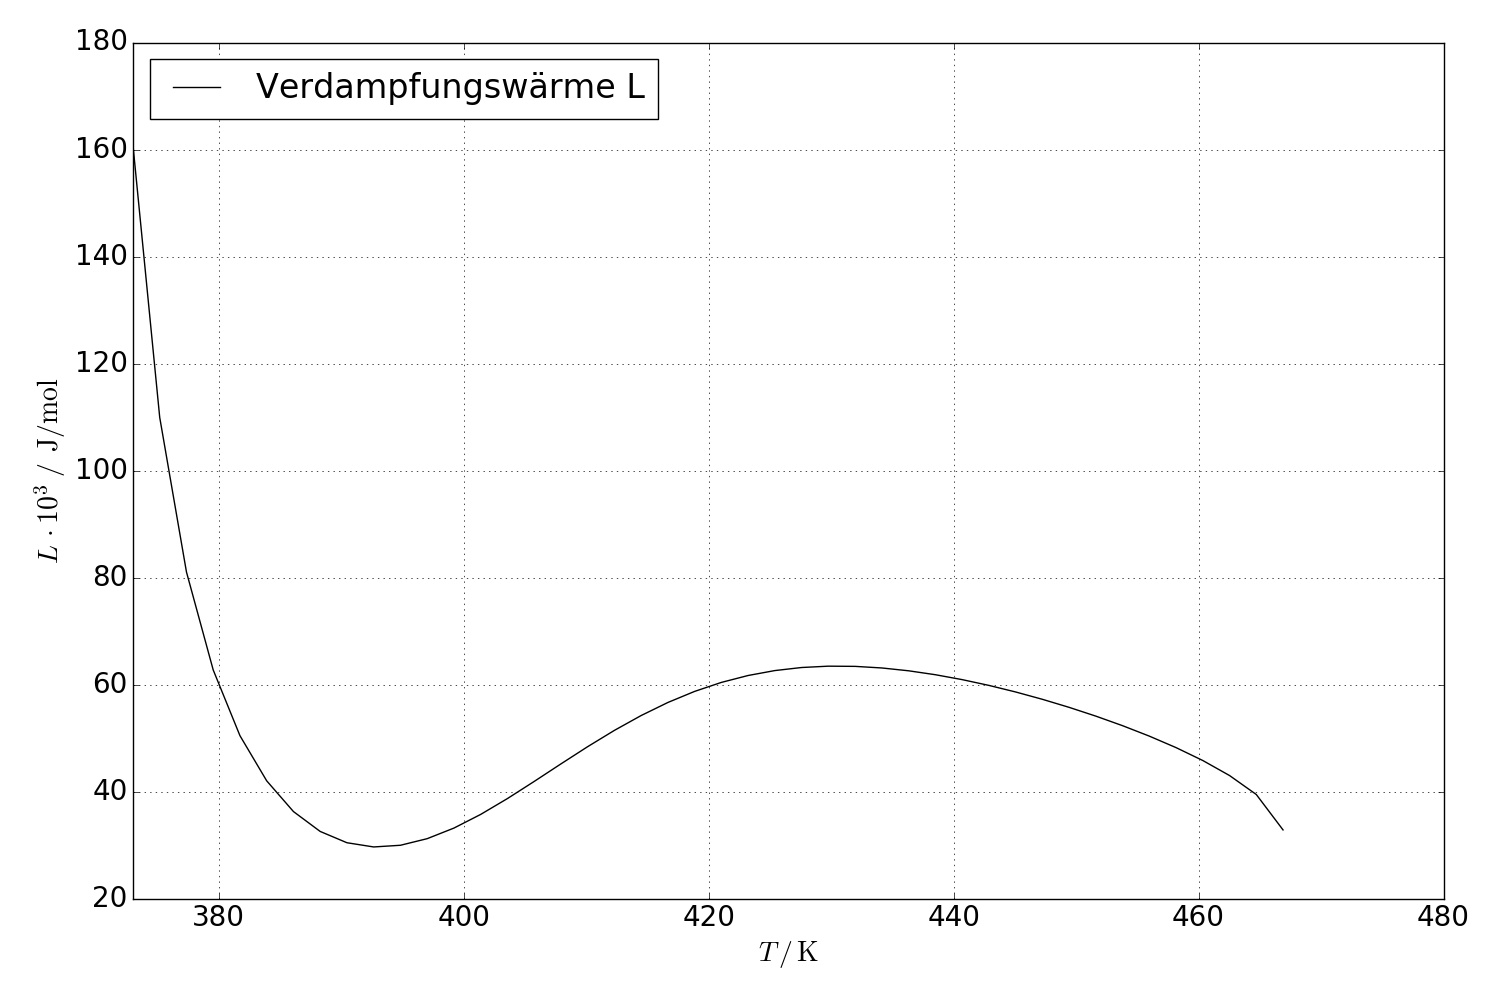
\includegraphics[height=5.5cm]{Lplus.jpg}
  \caption{Der Wurzelterm wird addiert}
  \label{fig:plus}
\end{figure}

\newpage
\section{Diskussion}
\section{Literaturverzeichnis}
\end{document}
